\documentclass[12pt, a4paper]{article}
\usepackage[french]{babel}
\usepackage{caption}
\usepackage{graphicx}
\usepackage[T1]{fontenc}
\usepackage{listings}
\usepackage{geometry}
\usepackage{pgfplots}
\pgfplotsset{width=10cm,compat=1.9}
% \usepackage[colorlinks=true,linkcolor=black,anchorcolor=black,citecolor=black,filecolor=black,menucolor=black,runcolor=black,urlcolor=black]{hyperref}
\usepackage{fancyhdr}
\pagestyle{fancy}
\lhead{}
\rhead{}
\chead{}
\rfoot{\thepage}
\lfoot{Martin Baumgaertner}
\cfoot{}

\renewcommand{\headrulewidth}{0.4pt}
\renewcommand{\footrulewidth}{0.4pt}

\begin{document}
\begin{titlepage}
	\newcommand{\HRule}{\rule{\linewidth}{0.5mm}} 
	\center 
	\textsc{\LARGE iut de colmar}\\[6.5cm] 
	\textsc{\Large R403 -- physique des télécoms}\\[0.5cm] 
	\textsc{\large Année 2022-23}\\[0.5cm]
	\HRule\\[0.75cm]
	{\Large\bfseries Etat de l'art et fabrication d'un antenne YAGI}\\[0.4cm]
	\HRule\\[1.5cm]
	\textsc{\large martin baumgaertner}\\[6cm] 

	\vfill\vfill\vfill
	{\large\today} 
	\vfill
\end{titlepage}
\newpage
\tableofcontents
\newpage
\section{Introduction}
\subsection{Définition}
L'antenne Yagi est un type d'antenne directive utilisée 
pour la réception et la transmission de signaux radio. 
Elle se compose de trois principaux éléments. Un reflecteur,
placé à l'opposé du sens de propagation, au milieu, 
un dipôle, puis un reflecteur qui lui permet d'orienter
le signal.\\

Voici un schéma réprésentatif d'une antenne Yagi :
\begin{figure}[h]
    \centering
    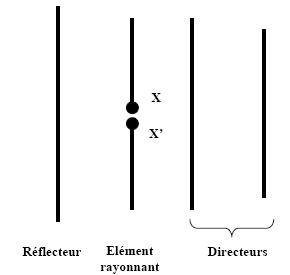
\includegraphics[width=0.5\textwidth]{img/yagi.jpg}
    \caption{Schéma d'une antenne Yagi \cite{r1}}
    \label{fig:yagi}
\end{figure}

\begin{figure}[h]
    \centering
    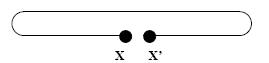
\includegraphics[width=0.5\textwidth]{img/trombone-yagi.jpg}
    \caption{Le dipôle vu de face \cite{r1}}
    \label{fig:yagi-de-face}
\end{figure}

Le dipôle peut être aussi appelé "trombone" en raison de sa
forme. Il est composé de deux éléments de même longueur. 
La longueur du dipôle est lié à la fréquence du signal
que l'on souhaite recevoir/émettre. En effet, la longueur
du dipôle doit être égale au quart de la longueur d'onde 
pour l'antenne Yagi la plus facile à réalisé : la quart d'onde.



\subsection{Présentation}

L'antenne Yagi, également connue sous le nom de 
"rateau", tire son nom de l'ingénieur japonais 
Shintaro Uda de l'université Tohoku à Sendai, qui 
l'a développée en collaboration avec son professeur 
Hidetsugu Yagi. En 1924, Uda conçut cette antenne 
directive, et la première publication sur sa découverte 
eut lieu en 1926 en japonais, puis en 1928 en anglais 
dans la revue scientifique "The Proceedings of the 
Institute of Radio Engineers" aux États-Unis. 
À partir de 1934, les radioamateurs ont commencé à
expérimenter cette antenne.\\

Pendant la Seconde Guerre. mondiale, l'antenne 
Yagi a été largement utilisée pour les radars.
Toutefois, c'est dans les années 1950, avec le
développement de la télévision, qu'elle s'est
répandue massivement sur les toits des habitations.
Elle est devenue populaire sous le nom
commun de "rateau", en raison de sa ressemblance.

Ainsi, l'antenne Yagi, de part son origine au Japon et
son utilisation répandue pendant la guerre et l'ère
de la télévision, a joué un rôle significatif dans
l'histoire des communications et continue d'être
utilisée de nos jours.\\

De nos jours les antennes Yagi sont principalement 
utilisées pour la réception de signaux de télévision
terrestre, pour la réception de signaux
radioamateurs et de téléphonie mobile. Ou bien même 
encore pour l'utilisation de Wi-Fi, bien installée, 
l'antenne permet de couvrir un bien plus grande surface 
qu'un petit modem. 


\section{Caractéristiques et propriétés des antennes Yagi}
\subsection{Fréquences et largeur de bande}
La largeur de bande des antennes Yagi est relative 
à l'utilisation que l'on en fait. En effet, la largeur 
de bande pour un réseau Wi-Fi sera bien plus grande
que celle d'une antenne de télévision. Voici quelques 
exemples de largeur de bande pour différentes 
utilisations :\\
\begin{itemize}
    \item Télévision numérique : 470-862 MHz 
    \item Réseaux Wi-Fi : 2,4-5,8 GHz
    \item Radioamateur : varie en fonction des bandes de fréquences souhaitées (HF, VHF, UHF)
\end{itemize}

\newpage
\subsection{Gain et directivité}
Le gain d'une antenne varie doit varier en fonction 
du nombre d'éléments qui la compose. En effet, plus
il y a d'éléments, plus le gain est important mais arrivé
à un certain point, le gain ne varie plus. Comme nous 
pouvons le voir ci-dessous, arrivé aux alentours 
de 20 élements on se rend compte que le gain commence
à stagner tout doucement. Il faut savoir adapter le nombre 
d'élements en fonction de ses besoins car \\ 


\begin{figure}
    \centering
    \begin{tikzpicture}
        \begin{axis}[	grid= major ,
                width=1\textwidth ,
                xlabel = {Nombre éléments} ,
                ylabel = {Gain(dBi)} ,
                xmin = 1, xmax = 26,
                ymin = 0, ymax = 20,
                legend entries={Évolution du gain},
                legend style={at={(0,1)},anchor=north west}]
            \addplot coordinates {(2, 6) (3, 8) (4, 9) (5, 10) (6, 11) (7, 12) (8, 13) (9, 13) (10, 14) (12, 14) (14, 15) (16, 15) (18, 16) (20, 16) (22, 17) (24, 17)}; % Tracé point à point
        \end{axis}
    \end{tikzpicture}
    \caption{Gain en fonction du nombre d'éléments \cite{r2}}
\end{figure}


\section{État de l'art des antennes Yagi}
\subsection{Principes de base}

\subsection{Avantages et limitations}




\section{Fabrication d'une antenne YAGI}
\subsection{Logiciels de conception et de simulation}

\subsection{Formules et équations utiles pour le dimensionnement}

\subsection{Outils et matériaux nécessaires}

\subsection{Fabrication de l'antenne - étapes par étapes}

\subsection{Exemples de projets de fabrication d'antennes Yagi}






\section{Conclusion}

\bibliographystyle{elsarticle-num}
\bibliography{rapport.bib}


\end{document}